% Chapter 4 — Integration on Manifolds (reviewed)
\chapter{Integration on Manifolds}

We shall consider integration of $p$-forms over differentiable singular $p$-chains in $n$-dimensional manifolds, and integration of $n$-forms over regular domains in oriented $n$-dimensional manifolds. For both of these situations we shall prove a version of Stokes' theorem. This is a generalization of the Fundamental Theorem of Calculus and is undoubtedly the single most important theorem in the subject. We shall also consider integration on Riemannian manifolds and on Lie groups. Finally, we shall introduce the de Rham cohomology groups and shall prove the Poincaré lemma, from which we will conclude that the de Rham cohomology groups of Euclidean space are trivial. This lemma will be of central importance for the de Rham theorem, which is stated at the end of this chapter and proved in Chapter 5.

\section{Orientation}


\begin{definition}\label{thm:4.1}
Let $V$ be a real vector space of dimension $n$. The notion of an orientation on $V$ was introduced in Exercise 13 of Chapter 2. Recall that the $n$th exterior power $\Lambda_n(V)$ is 1-dimensional, so that $\Lambda_n(V) - \{0\}$ has two components. An orientation on $V$ is a choice of a component of $\Lambda_n(V) - \{0\}$. \index{Orientation}

Now let $M$ be a connected differentiable manifold of dimension $n$. We shall call $M$ orientable if it is possible to choose in a consistent way an orientation on $M_m^*$ for each $m \in M$. More precisely, let $O$ be the “0-section” of the exterior $n$-bundle $\Lambda_n^*(M)$; that is,

\begin{equation}
\label{eq:4.1:1}
O=\bigcup_{m\in M}\left\{0\in\Lambda_{n}(M_{m}^{*})\right\}.
\end{equation}

Then since each $\Lambda_n(M_m^*) - \{0\}$ has exactly two components, it follows easily that $\Lambda_n^*(M) - O$ has at most two components. We say that $M$ is orientable if $\Lambda_n^*(M) - O$ has two components; and if $M$ is orientable, an orientation on $M$ is a choice of one of the two components of $\Lambda_n^*(M) - O$.

A non-connected manifold $M$ is said to be orientable if each component of $M$ is orientable, and an orientation is a choice of orientation on each component. Let $M$ be oriented, and let $v_{1}, \ldots, v_{n}$ be a basis of $M_{m}$ with dual basis $\delta_{1}, \ldots, \delta_{n}$. We say that the (ordered) basis $v_{1}, \ldots, v_{n}$ is oriented if $\delta_{1} \wedge \cdots \wedge \delta_{n}$ belongs to the orientation.

Let $M$ and $N$ be orientable $n$-dimensional manifolds, and let $\psi: M \to N$ be a differentiable map. We say that $\psi$ preserves orientations if the induced map $\delta\psi: \Lambda_n^*(N) \to \Lambda_n^*(M)$ maps the component of $\Lambda_n^*(N) - O$ determining the orientation on $N$ into the component of $\Lambda_n^*(M) - O$ determining the orientation on $M$. Equivalently, $\psi$ is orientation-preserving if $d\psi$ sends oriented bases of the tangent spaces to $M$ into oriented bases of the tangent spaces to $N$.

\end{definition}

\begin{proposition}\label{thm:4.2}
Let M be a differentiable manifold of dimension n. Then the following are equivalent:

(a) M is orientable.

(b) There is a collection $\Phi = \{(V,\psi)\}$ of coordinate systems on $M$ such that

\begin{equation}
\label{eq:4.2:1}
M=\bigcup_{(V,\psi)\in\Phi}V\qquad\mathrm{and}\qquad\det\left(\frac{\partial x_{i}}{\partial y_{j}}\right)>0\quad\mathrm{on}\quad U\cap V
\end{equation}

whenever $(U, x_{1}, \ldots, x_{n})$ and $(V, y_{1}, \ldots, y_{n})$ belong to $\Phi$.

(c) There is a nowhere-vanishing n-form on M.

\end{proposition}

\begin{proof}
We can assume, without loss of generality, that $M$ is connected. We prove that (a) $\Rightarrow$ (b) $\Rightarrow$ (c) $\Rightarrow$ (a). Given (a), that $M$ is orientable, choose an orientation on $M$; that is, we choose one of the two components, call it $\Lambda$, of $\Lambda_n^*(M) - O$. Observe that for each $m \in M$, $\Lambda \cap \Lambda_n(M_m^*)$ is precisely one of the two components of $\Lambda_n(M_m^*) - \{0\}$. Now let $\Phi$ consist of all of those coordinate systems $(V, y_1, \ldots, y_n)$ on $M$ such that the map of $V$ into $\Lambda_n^*(M)$ defined by

\begin{equation}
\label{eq:4.2:2}
m\mapsto(d y_{1}\land\cdots\land d y_{n})(m)
\end{equation}

has range in $\Lambda$. Now, if $(U, x_1, \ldots, x_n)$ and $(V, y_1, \ldots, y_n)$ are any two coordinate systems on $M$, then for $m \in U \cap V$,

\begin{equation}
\label{eq:4.2:3}
(d x_{1}\wedge\dotsm\wedge d x_{n})(m)=\det\biggl(\frac{\partial x_{i}}{\partial y_{j}}\bigg|_{m}\biggr)(d y_{1}\wedge\dotsm\wedge d y_{n})(m).
\end{equation}

If these coordinate systems belong to $\Phi$, then necessarily

\[
\det\left(\frac{\partial x_{i}}{\partial y_{j}}\bigg|_{m}\right)>0
\]

for each $m \in U \cap V$. Consequently, (1) is satisfied, and result (b) follows from (a).

Now assume (b). Let $\{\varphi_i\}$ be a partition of unity subordinate to the cover of $M$ given by the coordinate neighborhoods in the collection $\Phi$ with $\varphi_i$ subordinate to $(V_i, x_1^i, \ldots, x_n^i)$. Then

\begin{equation}
\label{eq:4.2:4}
\omega=\sum_{i}\varphi_{i}d x_{1}{}^{i}\wedge\cdots\wedge d x_{n}{}^{i}
\end{equation}

is a global $n$-form on $M$, where $\varphi_i \, dx_1^i \wedge \cdots \wedge dx_n^i$ is defined to be the $0$-form outside of $V_i$. That $\omega$ vanishes nowhere follows from the fact that for each $m$, $\omega(m)$ is a finite sum with positive coefficients of elements of one component of $\Lambda_n(M_m^*) - \{0\}$. Thus (c) follows from (b).

Finally, let  $ \omega $ be a nowhere-vanishing n-form on M, and let

\[
\Lambda^{+}=\bigcup_{m\in M}\{a\omega(m)\colon a\in\mathbb{R},a>0\},
\]

\[
\Lambda^{-}=\bigcup_{m\in M}\{a\omega(m)\colon a\in\mathbb{R},\;a<0\}.
\]

Then  $ \Lambda_n^*(M) - O $ is the disjoint union of the two open subsets  $ \Lambda^+ $ and  $ \Lambda^- $, so  $ \Lambda_n^*(M) - O $ is disconnected, and  $ M $ is orientable.

\end{proof}

\begin{examples}\label{thm:4.3}
(a) Every Lie group $G$ is orientable, for if $\omega_1, \ldots, \omega_n$ is a basis for the left invariant 1-forms on $G$, then $\omega_1 \wedge \cdots \wedge \omega_n$ is a global nowhere-vanishing $n$-form on $G$.

(b) The standard orientation on the Euclidean space  $ \mathbb{R}^d $ is the one determined by the  $ d $-form  $ dr_1 \wedge \cdots \wedge dr_d $.

(c) Let $X$ be a $d$-dimensional manifold, and suppose that there exists an immersion $f: X \to \mathbb{R}^{d+1}$. A normal vector field along $(X, f)$ is a smooth map $N: X \to T(\mathbb{R}^{d+1})$ such that for each $p \in X$, the vector $N(p)$ lies in $(\mathbb{R}^{d+1})_{f(p)}$ and is orthogonal to the subspace $df(X_p) \subset (\mathbb{R}^{d+1})_{f(p)}$. Such a manifold $X$ is orientable if and only if there is a smooth nowhere-vanishing normal vector field along $(X, f)$. (See Exercise 1.)

(d) As an immediate application of Example (c), the sphere $S^{n}$ is orientable for each  $ n \geq 1 $.

(e) The real projective space  $ P^n $ is orientable if and only if n is odd. (See Exercise 2.)

\end{examples}

\section{Integration on Manifolds}


\subsection{Integration in the Euclidean Space $\mathbb{R}^n$}\label{thm:4.4}
We assume that the reader is familiar with some theory of integration in  $ \mathbb{R}^n $. Since we shall be integrating continuous (in fact usually  $ C^\infty $) functions over nice subsets of  $ \mathbb{R}^n $ \index{Integration}

(polyhedra for example), the theory of the Riemann integral will be quite sufficient. The principal theorem that we need to recall is the change of variables formula. Several versions of this formula and their proofs may be found in [6], [18], or [29]. A version sufficient for our purposes is the following. Let $\varphi$ be a diffeomorphism of a bounded open set $D$ in $\mathbb{R}^{n}$ with a bounded open set $\varphi(D)$. Let $J_{\varphi}$ denote the determinant of the Jacobian matrix of $\varphi$:

\[
J_{\varphi}=\det\left(\frac{\partial\varphi_{i}}{\partial r_{j}}\right)\;.
\]

Let $f$ be a bounded continuous function on $\varphi(D)$, and let $A$ be a nice subset of $D$. ($A$ will be polyhedral in most of our applications. Generally, for the Riemann theory, a nice subset would be one which has Jordan content.) Then

\begin{equation}
\label{eq:4.4:1}
\int_{\varphi(A)}f=\int_{A}f\circ\varphi\,|J_{\varphi}|.
\end{equation}

\subsection{Integration of $n$-forms in $\mathbb{R}^n$}\label{thm:4.5}
As usual, we let $r_1, \ldots, r_n$ denote the canonical coordinate system on $\mathbb{R}^n$. The standard orientation is determined by the $n$-form $dr_1 \wedge \cdots \wedge dr_n$. Now let $\omega$ be an $n$-form on an open set $D \subset \mathbb{R}^n$. Then there is a uniquely determined function $f$ on $D$ such that $\omega = f dr_1 \wedge \cdots \wedge dr_n$. Let $A \subset D$. We define

\begin{equation}
\label{eq:4.5:1}
\int_{A}\omega=\int_{A}f,
\end{equation}

provided that the latter exists. We can restate the change of variables formula \eqref{eq:4.4:1} in terms of differential forms. Let $\varphi$, $D$, and $A$ be as in 4.4, and let $\omega$ be an $n$-form on $\varphi(D)$. Then

\begin{equation}
\label{eq:4.5:2}
\int_{\varphi(A)}\omega=\pm\int_{A}\delta\varphi(\omega),
\end{equation}

where one uses “+” if φ is orientation preserving and “−” if φ is orientation reversing.

\subsection{Integration over Chains}\label{thm:4.6}
The first type of integration that we shall consider on general manifolds involves integration of $p$-forms over differentiable singular $p$-chains in an $n$-manifold.

For each  $ p \geq 1 $ we let

\begin{equation}
\label{eq:4.6:1}
\Delta^{p}=\Big\{(a_{1},\ldots,a_{p})\in\mathbb{R}^{p}\colon\sum_{i=1}^{p}a_{i}\leq1,\mathrm{and~each}a_{i}\geq0\Big\}.
\end{equation}

$\Delta^{p}$ is called the standard $p$-simplex in $\mathbb{R}^{p}$. For $p=0$, we set $\Delta^{p}$ equal to the $1$-point space $\{0\}$; $\Delta^{p}$ is the standard $0$-simplex. Let $M$ be a manifold. A differentiable singular $p$-simplex $\sigma$ in $M$ is a map $\sigma$ of $\Delta^{p}$ into $M$ which extends to be a differentiable $(C^{\infty})$ map of a neighborhood of $\Delta^{p}$ in $\mathbb{R}^{p}$ into $M$. \index{Simplex}

In this chapter we shall refer to such a $\sigma$ as simply a $p$-simplex $\sigma$ in $M$. (In Chapter 5 we shall deal, in addition, with continuous singular simplices, and so there we shall need to retain the term “differentiable” for distinction.) A $0$-simplex in $M$ consists of a map of the 1-point space $\{0\}$ into $M$. $\mathbf{A}p$-chain $c$ in $M$ (with real coefficients) is a finite linear combination $c=\sum a_i\sigma_i$ of $p$-simplices $\sigma_i$ in $M$ where the $a_i$ are real numbers. \index{Chain}

For each $p \geq 0$ we define a collection of maps $k_i^{p}: \Delta^{p} \to \Delta^{p+1}$ for $0 \leq i \leq p + 1$ as follows:

\[
\mathrm{f o r}\quad p=0,\quad k_{0}^{0}(0)=1\quad\mathrm{a n d}\quad k_{1}^{0}(0)=0.
\]

\begin{equation}
\label{eq:4.6:2}
\begin{array}{l l}{\mathrm{f o r}\quad p\geq1,}&{\begin{cases}{k_{0}^{p}(a_{1},\ldots,a_{p})=\left(1-\sum_{i=1}^{p}a_{i},a_{1},\ldots,a_{p}\right)\quad\mathrm{and}}\\ {k_{i}^{p}(a_{1},\ldots,a_{p})=(a_{1},\ldots,a_{i-1},0,a_{i},\ldots,a_{p})}\\ {\quad(1\leq i\leq p+1).}\\ \end{cases}}\\ \end{array}
\end{equation}

If  $ \sigma $ is a  $ p $-simplex in  $ M $ with  $ p \geq 1 $, we define its  $ ith $ face,  $ 0 \leq i \leq p $, to be the  $ (p-1) $-simplex

\begin{equation}
\label{eq:4.6:3}
\sigma^{i}=\sigma\circ k_{i}^{p-1},
\end{equation}

and we define the boundary of  $ \sigma $ to be the  $ (p - 1) $ chain

\begin{equation}
\label{eq:4.6:4}
\partial\sigma=\sum_{i=0}^{p}(-1)^{i}\sigma^{i}.
\end{equation}

We extend the boundary operator linearly to chains. Note carefully the use of the superscript to denote faces. Thus the boundary of the $p$-chain $\sum_{i=1}^{k}a_{i}\sigma_{i}$ is

\[
\sum_{i=0}^{p}\sum_{j=1}^{k}(-1)^{i}a_{j}\sigma_{j}^{i}.
\]

\begin{center}
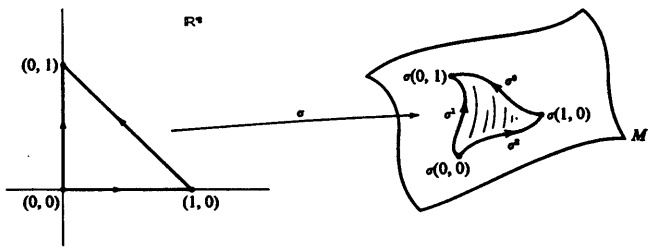
\includegraphics[width=0.60\textwidth]{figures/ch4_img_in_image_box_125_823_775_1072.jpg}
\end{center}

We claim that

\begin{equation}
\label{eq:4.6:5}
k_{i}^{p+1}\circ k_{j}^{p}=k_{j+1}^{p+1}\circ k_{i}^{p}\qquad(p\geq0;i\leq j).
\end{equation}

For $p=0$, check the three possible cases separately. For $p\geq1$, observe that both sides of (5) give the following maps:

\begin{equation}
\label{eq:4.6:6}
\begin{aligned}{}&{{}\quad1\leq i<j\quad(a_{1},\ldots,a_{p})\mapsto(a_{1},\ldots,a_{i-1},0,a_{i},\ldots,a_{j-1},0,a_{j},\ldots,a_{p})}\\ {}&{{}\quad1\leq i=j\quad(a_{1},\ldots,a_{p})\mapsto(a_{1},\ldots,a_{i-1},0,0,a_{i},\ldots,a_{p})}\\ {}&{{}\quad0=i<j\quad(a_{1},\ldots,a_{p})\mapsto\bigg(1-\sum_{i=1}^{p}a_{i},a_{1},\ldots,a_{j-1},0,a_{j},\ldots,a_{p}\bigg)}\\ {}&{{}\quad0=i=j\quad(a_{1},\ldots,a_{p})\mapsto\bigg(0,1-\sum_{i=1}^{p}a_{i},a_{1},\ldots,a_{p}\bigg).}\\ \end{aligned}
\end{equation}

It follows from (5), (3), and (4) that the boundary of the boundary of a chain is always 0. That is,

\begin{equation}
\label{eq:4.6:7}
\partial\circ\partial=0.
\end{equation}

Now let $\sigma$ be a $p$-simplex in $M$, and let $\omega$ be a $p$-form defined on a neighborhood of the image of $\sigma$. In most of our applications we shall deal only with smooth forms, but for the purposes of the following definition it would be quite sufficient for $\omega$ to be a continuous $p$-form. First of all, if $p = 0$, then a 0-simplex consists simply of a point in $M$, and a 0-form is simply a function. In this case, we define the integral of the function $\omega$ over the 0-simplex $\sigma$ to be the value of $\omega$ at the point $\sigma(0) \in M$:

\begin{equation}
\label{eq:4.6:8}
\int_{\sigma}\omega=\omega\left(\sigma(0)\right).
\end{equation}

If $p \geq 1$, then since $\sigma$ extends to be a smooth map of a neighborhood of $\Delta^p$ in $\mathbb{R}^p$ into $M$, $\omega$ can be pulled back via $\sigma$ to a $p$-form $\delta\sigma(\omega)$ on a neighborhood of $\Delta^p$. In this case, we define the integral of the $p$-form $\omega$ over the $p$-simplex $\sigma$ by

\begin{equation}
\label{eq:4.6:9}
\int_{\sigma}\omega=\int_{\Delta^{p}}\delta\sigma(\omega).
\end{equation}

We extend these integrals linearly to chains, so that if  $ c = \sum a_i \sigma_i $, then

\begin{equation}
\label{eq:4.6:10}
\int_{c}\omega=\sum a_{i}\int_{\sigma_{i}}\omega.
\end{equation}

Perhaps the single most important theorem in integration theory on manifolds is Stokes' theorem. This is a generalization of the Fundamental Theorem of Calculus. Observe that in our context the Fundamental Theorem says that if $F$ is a smooth function on the real line, and if $\sigma$ is a smooth 1-simplex in the real line, then

\begin{equation}
\label{eq:4.6:11}
\int_{\partial\sigma}F=\int_{\sigma}dF.
\end{equation}

We shall present two versions of Stokes' theorem. The first is in terms of integration of forms over chains. \index{Stokes' theorem}

\begin{theorem}{Stokes' Theorem I}\label{thm:4.7}
Let $c$ be a $p$-chain ($p \geq 1$) in a differentiable manifold $M$, and let $\omega$ be a smooth ($p-1$) form defined on a neighborhood of the image of $c$. Then

\begin{equation}
\label{eq:4.7:1}
\int_{\partial c}\omega=\int_{c}d\omega.
\end{equation}

\end{theorem}

\begin{proof}
It is sufficient to consider the case in which the p-chain c consists of a single p-simplex  $ \sigma $. Thus we must prove that

\begin{equation}
\label{eq:4.7:2}
\int_{\sigma}d\omega=\int_{\partial\sigma}\omega.
\end{equation}

It follows immediately from our definitions that (2) is equivalent with

\begin{equation}
\label{eq:4.7:3}
\int_{\Delta^{p}}d\left(\delta\sigma(\omega)\right)=\sum_{i=0}^{p}(-1)^{i}\int_{\Delta^{p-1}}\delta\sigma^{i}(\omega)=\sum_{i=0}^{p}(-1)^{i}\int_{\Delta^{p-1}}\delta k_{i}^{p-1}\circ\delta\sigma(\omega).
\end{equation}

Observe first of all that the case p = 1 reduces directly to the Fundamental Theorem of Calculus:

\begin{equation}
\label{eq:4.7:4}
\int_{\Delta^{1}}\frac{d}{d r}(\omega\circ\sigma)d r=\omega\big(\sigma(1)\big)-\omega\big(\sigma(0)\big),
\end{equation}

so we now assume that  $ p \geq 2 $. Then the  $ (p - 1) $ form  $ \delta\sigma(\omega) $ can be expressed as

\begin{equation}
\label{eq:4.7:5}
\delta\sigma(\omega)=\sum_{j=1}^{p}a_{j}\,dr_{1}\wedge\cdots\wedge\widehat{dr_{j}}\wedge\cdots\wedge dr_{p},
\end{equation}

where the circumflex over a term means that the term is to be omitted, and where the $a_i$ are $C^\infty$ functions on a neighborhood of $\Delta^p$ in $\mathbb{R}^p$. Since the integral is linear, we may consider the special case in which $\delta\sigma(\omega)$ consists of a single term of the form $a_i dr_1 \wedge \cdots \wedge \widehat{dr}_j \wedge \cdots \wedge dr_p$. In this case, the left-hand side of (3) becomes

\begin{equation}
\label{eq:4.7:6}
(-1)^{j-1}\int_{\Delta^{p}}\frac{\partial a_{j}}{\partial r_{j}}d r_{1}\wedge\cdots\wedge d r_{p}.
\end{equation}

To evaluate the right-hand side of (3), we observe that for  $ 1 \leq i \leq p $,

\begin{equation}
\label{eq:4.7:7}
\delta k_{i}^{p-1}(r_{j})=\left\{\begin{matrix}{r_{j}}&{}&{(1\leq j\leq i-1)}\\ {0}&{}&{(j=i)}\\ {r_{j-1}}&{}&{(i+1\leq j\leq p),}\\ \end{matrix}\right.
\end{equation}

and

\begin{equation}
\label{eq:4.7:8}
\delta k_{0}^{p-1}(r_{j})=\left\{\begin{aligned}{}&{{}1-\sum_{i=1}^{p-1}r_{i}}&{(j=1)}\\ {}&{{}r_{j-1}}&{(1<j\leq p).}\\ \end{aligned}\right.
\end{equation}

Applying (7) and (8) to the right-hand term of (3), we obtain


\begin{align*}\sum_{i=0}^{p}(-1)^{i}&\int_{\Delta^{p-1}}\delta k_{i}^{p-1}(a_{j} dr_{1}\wedge\cdots\wedge\widehat{dr}_{j}\wedge\cdots\wedge dr_{p})\\&=(-1)^{j-1}\int_{\Delta^{p-1}}a_{j}\bigg(1-\sum_{i=1}^{p-1}r_{i},r_{1},\ldots,r_{p-1}\bigg)dr_{1}\wedge\cdots\wedge dr_{p-1}\\&\quad+(-1)^{j}\int_{\Delta^{p-1}}a_{j}(r_{1},\ldots,r_{j-1},0,r_{j},\ldots,r_{p-1})dr_{1}\wedge\cdots\wedge dr_{p-1}.\end{align*}


We shall now apply a change of variables to the first term on the right-hand side of (9). Let $\varphi_{j}$ be the diffeomorphism of $\mathbb{R}^{p-1}$ defined by

\[
\varphi_{j}(r_{1},\ldots,r_{p-1})=\begin{cases}{(r_{1},\ldots,r_{p-1})}&{(j=1)}\\ {\left(1-\displaystyle\sum_{i=1}^{p-1}r_{i},r_{2},\ldots,r_{p-1}\right)}&{(j=2)}\\ {\left(r_{2},\ldots,r_{j-1},1-\displaystyle\sum_{i=1}^{p-1}r_{i},r_{j},\ldots,r_{p-1}\right)}&{}\\ {\quad(3\leq j\leq p).}\\ \end{cases}
\]

Then  $\varphi_j(\Delta^{p-1}) = \Delta^{p-1}$, and $|J_{\varphi_j}| = 1$, so that by \eqref{eq:4.4:1}, the first term on the right-hand side of (9) is equal to

\[
(-1)^{i-1}\int_{\Delta^{p-1}}a_{j}\left(r_{1},\ldots,r_{j-1},1-\sum_{i=1}^{p-1}r_{i},r_{j},\ldots,r_{p-1}\right)d r_{1}\wedge\cdots\wedge d r_{p-1}.
\]

From (3), (6), (9), and (11) we see that the proof has been reduced to showing that

\begin{equation}
\label{eq:4.7:9}
\begin{aligned}{}&{{}\int_{\Delta^{p}}\frac{\partial a_{j}}{\partial r_{j}}d r_{1}\wedge\cdots\wedge d r_{p}}\\ {}&{{}\quad=\int_{\Delta^{p-1}}a_{j}\bigg(r_{1},\ldots,r_{j-1},1-\sum_{i=1}^{p-1}r_{i},r_{j},\ldots,r_{p-1}\bigg)d r_{1}\wedge\cdots\wedge d r_{p-1}}\\ {}&{{}\quad-\int_{\Delta^{p-1}}a_{j}(r_{1},\ldots,r_{j-1},0,r_{j},\ldots,r_{p-1})d r_{1}\wedge\cdots\wedge d r_{p-1}.}\\ \end{aligned}
\end{equation}

But now (12) is simply the evaluation of the integral of $\partial a_{i}/\partial r_{i}$ over $\Delta^{p}$ by iterating first with respect to $r_{i}$ and applying again the Fundamental Theorem of Calculus.

\end{proof}

\subsection{Integration on an Oriented Manifold}\label{thm:4.8}
Let $M$ be an $n$-dimensional oriented manifold. We shall integrate $n$-forms over regular domains in $M$. A subset $D$ of $M$ will be called a regular domain if for each point $m \in M$ one of the following holds: \index{Regular domain}

(a) There is an open neighborhood of m which is contained in M - D.

(b) There is an open neighborhood of m which is contained in D.

(c) There is a centered coordinate system $(U,\varphi)$ about $m$ such that $\varphi(U\cap D)=\varphi(U)\cap H^n$, where $H^n$ is the half-space of $\mathbb{R}^n$ defined by $r_n\geq0$.

Points of $D$ of type (b) are called interior points and comprise the interior, Int(D), of $D$. Points of type (c) are called boundary points and comprise the boundary, $\partial D$, of $D$. Coordinate systems of type (c) restricted to $\partial D$ overlap differentiably and yield a manifold structure of dimension $n-1$ on $\partial D$, making $\partial D$ into an imbedded $(n-1)$ dimensional submanifold of $M$.

Let $m \in \partial D$, and let $v \in M_m$. We call $v$ an outer vector to $D$ if there is a smooth curve $\alpha(t)$ in $M$ with $\dot{\alpha}(0) = v$ and with $\alpha(t) \notin D$ for $0 < t < \varepsilon$, for some $\varepsilon > 0$. The orientation on $M$ induces an orientation on $\partial D$ as follows. Let $v$ be an outer vector to $D$ at $m$, and let $v_1, \ldots, v_{n-1}$ be a basis of the tangent space $(\partial D)_m$. Then we define $v_1, \ldots, v_{n-1}$ to be an oriented basis of $(\partial D)_m$ if and only if $v, v_1, \ldots, v_{n-1}$ is an oriented basis of $M_m$. One can easily check that this definition is independent of the outer vector $v$ chosen, and that this defines a smooth orientation on $\partial D$ in the sense of 4.1.

Now let $\omega$ be an $n$-form ($n = \dim M$) with compact support, and let $D$ be a regular domain in $M$. As a particular case, $D$ could be all of $M$. We are going to define the integral of $\omega$ over $D$. As in 4.6, it will be sufficient for the purposes of this definition for $\omega$ to be a continuous $n$-form. We shall use a partition of unity to reduce the support of $\omega$ to certain $n$-simplices in $M$ over which we can integrate as in \eqref{eq:4.6:9}. First, we shall choose some $n$-simplices suitably related to $D$ and $\partial D$.

An $n$-simplex $\sigma$ in $M$ will be called regular if $\sigma$ extends to a diffeomorphism on a neighborhood of $\Delta^n$. When speaking of regular $n$-simplices, we shall always assume that they have been extended in this way to a neighborhood of $\Delta^n$. An oriented regular $n$-simplex is one in which the map $\sigma$ preserves orientations. (We always take the standard orientation on $\mathbb{R}^n$.)

Associated with a given regular domain $D$, we shall consider only oriented regular $n$-simplices of the following two types:

$ (\alpha) $  $ \sigma(\Delta^n) \subset \operatorname{Int}(D) $.

$ (\beta) $  $ \sigma(\Delta^n) \subset D $ and  $ \sigma(\Delta^n) \cap \partial D = \sigma^n (\Delta^{n-1}) $; that is, precisely the nth face of  $ \sigma $ lies in the boundary of  $ D $.

Now cover D by open sets U of the following types:

$ (\alpha') \quad U $ lies in the interior of an oriented regular  $ n $-simplex  $ \sigma $ of type  $ (\alpha) $.

$ (\beta') $ U is the image under a type  $ (\beta) $ oriented regular  $ n $-simplex  $ \sigma $ of an open set  $ V $ in  $ \mathbb{R}^n $ which is a neighborhood of a point in the  $ n $th face of  $ \Delta^n $, which intersects the boundary of  $ \Delta^n $ only in that  $ n $th face, and whose image under  $ \sigma $ is contained in  $ \sigma(\Delta^n) \cup (M - D) $.

\begin{center}
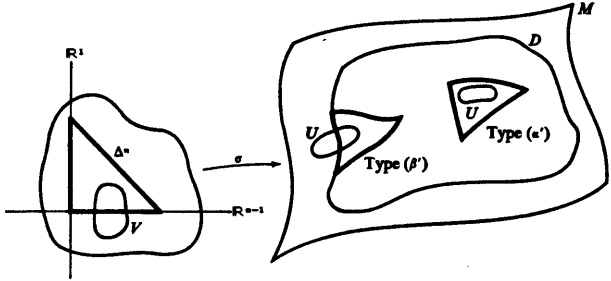
\includegraphics[width=0.60\textwidth]{figures/ch4_img_in_image_box_158_107_769_388.jpg}
\end{center}

Since supp $\omega \cap D$ is compact, it has a finite cover $U_1, \ldots, U_k$ by open sets of type $(\alpha')$ or $(\beta')$. Let the associated oriented regular $n$-simplices be $\sigma_1, \ldots, \sigma_k$. Let $U = M - (\text{supp} \omega \cap D)$, and let $\varphi, \varphi_1, \ldots, \varphi_k$ be a partition of unity subordinate to the cover $U, U_1, \ldots, U_k$ of $M$. We define the integral of $\omega$ over $D$ by

\begin{equation}
\label{eq:4.8:1}
\int_{D}\omega=\sum_{i=1}^{k}\int_{\sigma_{i}}\varphi_{i}\omega.
\end{equation}

We must check that the definition (1) is independent of the cover and the partition of unity chosen. Let $V, V_{1}, \ldots, V_{l}$ and $\psi, \psi_{1}, \ldots, \psi_{l}$ be another such cover and another such partition of unity respectively, with $V_{j}$ associated with the oriented regular $n$-simplex $\tau_{j}$. Since $\psi = 0$ on $\mathrm{supp} \omega \cap D$, it follows that $\sum_{j=1}^{l}\psi_{j} = 1$ there, so that

\begin{equation}
\label{eq:4.8:2}
\sum_{i=1}^{k}\int_{\sigma_{i}}\varphi_{i}\omega=\sum_{i=1}^{k}\int_{\sigma_{i}}\sum_{j=1}^{l}\psi_{j}\varphi_{i}\omega=\sum_{i,j}\int_{\sigma_{i}}\psi_{j}\varphi_{i}\omega.
\end{equation}

Similarly,

\begin{equation}
\label{eq:4.8:3}
\sum_{j=1}^{l}\int_{\tau_{j}}\psi_{j}\omega=\sum_{i,j}\int_{\tau_{j}}\psi_{j}\varphi_{i}\omega.
\end{equation}

Now, since $\sigma_i^{-1}\circ\tau_j$ is an orientation-preserving diffeomorphism on the open set (possibly empty) where it is defined, and since (supp $\psi_j\varphi_i\omega$) $\cap\sigma_i(\Delta^n) = (\mathrm{supp}\,\psi_j\varphi_i\omega)\cap\tau_j(\Delta^n)$, it follows from the change of variables formula \eqref{eq:4.5:2} that

\begin{equation}
\label{eq:4.8:4}
\begin{aligned}{\int_{\sigma_{i}}\psi_{j}\varphi_{i}\omega=}&{{}\int_{\Delta^{n}}\delta\sigma_{i}(\psi_{j}\varphi_{i}\omega)=\int_{\Delta^{n}}\delta(\sigma_{i}^{-1}\circ\tau_{j})[\delta\sigma_{i}(\psi_{j}\varphi_{i}\omega)]}\\ {=}&{{}\int_{\Delta^{n}}\delta\tau_{j}(\psi_{j}\varphi_{i}\omega)=\int_{\tau_{j}}\psi_{j}\varphi_{i}\omega.}\\ \end{aligned}
\end{equation}

It follows from (2), (3), and (4) that $\int_{D} \omega$ is well-defined, independent of the choice of cover and partition of unity.

Observe that if $\gamma$ is a diffeomorphism of $M$, then

\begin{equation}
\label{eq:4.8:5}
\int_{\gamma(D)}\omega=\pm\int_{D}\delta\gamma(\omega)
\end{equation}

with “+” if and only if  $ \gamma $ is orientation-preserving.

We now are ready to state and prove our second version of Stokes' theorem.

\begin{theorem}{Stokes' Theorem II}\label{thm:4.9}
Let $D$ be a regular domain in an oriented $n$-dimensional manifold $M$, and let $\omega$ be a smooth $(n-1)$ form of compact support. Then

\begin{equation}
\label{eq:4.9:1}
\int_{D}d\omega=\int_{\partial D}\omega.
\end{equation}

\end{theorem}

\begin{proof}
Let $\varphi_{1},\ldots,\varphi_{k}$ and $\sigma_{1},\ldots,\sigma_{k}$ be chosen as in \eqref{eq:4.8:1} relative to (supp $\omega$) $\cap D$. Since $\sum_{i=1}^{k}\varphi_{i}=1$ on a neighborhood of (supp $\omega$) $\cap D$, $d(\sum\varphi_{i})=0$ there. Thus on a neighborhood of (supp $\omega$) $\cap D$ we have

\begin{equation}
\label{eq:4.9:2}
\sum_{i=1}^{k}d(\varphi_{i}\omega)=\sum_{i=1}^{k}d\varphi_{i}\wedge\omega+\sum_{i=1}^{k}\varphi_{i}d\omega=d\omega.
\end{equation}

Now, if $\sigma_{i}$ is an $n$-simplex of type 4.8( $ \alpha $), then

\begin{equation}
\label{eq:4.9:3}
\int_{\partial\sigma_{i}}\varphi_{i}\omega=0=\int_{\partial D}\varphi_{i}\omega
\end{equation}

since $\mathrm{supp} \ \varphi_i \omega \subset \mathrm{Int} \ \sigma_i(\Delta^n) \subset \mathrm{Int} \, D$. On the other hand, suppose that $\sigma_i$ is an $n$-simplex of type 4.8($\beta$). In this case, $\varphi_i \omega$ is zero on the boundary of $\sigma_i$ except possibly at points in the interior of the $n$th face $\sigma_i^n$. Now $\sigma_i^n$ is an orientation-preserving regular ($n-1$) simplex in $\partial D$ if $n$ is even, and is orientation-reversing if $n$ is odd. It follows that

\begin{equation}
\label{eq:4.9:4}
\int_{\partial\sigma_{i}}\varphi_{i}\omega=(-1)^{n}\int_{\sigma_{i}{}^{n}}\varphi_{i}\omega=(-1)^{n}(-1)^{n}\int_{\partial D}\varphi_{i}\omega=\int_{\partial D}\varphi_{i}\omega.
\end{equation}

From (2), (3), (4), and from our first version (4.7) of Stokes' theorem, we see that

\begin{equation}
\label{eq:4.9:5}
\begin{aligned}{\int_{D}d\omega}&{{}=\sum_{i}\int_{D}d(\varphi_{i}\omega)=\sum_{i}\int_{\sigma_{i}}d(\varphi_{i}\omega)}\\ {}&{{}=\sum_{i}\int_{\partial\sigma_{i}}\varphi_{i}\omega=\sum_{i}\int_{\partial D}\varphi_{i}\omega=\int_{\partial D}\omega.}\\ \end{aligned}
\end{equation}

\end{proof}

\begin{corollary*}
Let $\omega$ be a smooth $(n-1)$ form on a compact oriented $n$-dimensional manifold $M$. Then

\[
\int_M d\omega=0.
\]

\end{corollary*}

\subsection{Integration on a Riemannian Manifold}\label{thm:4.10} Let $M$ be a Riemannian manifold of dimension $n$. That is, $M$ is an $n$-dimensional differentiable manifold with a positive definite inner product $\langle \ , \rangle_m$ on each tangent space $M_m$ such that $m \mapsto \langle X, Y \rangle_m$ is a smooth function on $M$ whenever $X$ and $Y$ are smooth vector fields. The existence of Riemannian metrics on differentiable manifolds was asserted in Exercise 23 of Chapter 1.

Given a point  $ m \in M $, one can find a neighborhood  $ U $ of  $ m $ and a collection  $ e_1, \ldots, e_n $ of  $ C^\infty $ vector fields on  $ U $ which are orthonormal in the sense that they form an orthonormal basis of the tangent space to  $ M $ at each point of  $ U $. Start with a coordinate neighborhood  $ (U, x_1, \ldots, x_n) $, apply the usual Gram-Schmidt procedure to orthonormalize the vector fields  $ \partial/\partial x_1, \ldots, \partial/\partial x_n $, and do it simultaneously at all points of  $ U $. Such a collection  $ e_1, \ldots, e_n $ is called a local orthonormal frame field. \index{Frame field}

Since the inner product  $ \langle \quad, \quad\rangle_{m} $ is, in particular, a non-singular pairing of  $ M_{m} $ with itself, it induces (see 2.7) a natural isomorphism of  $ M_{m} $ with  $ M_{m}^{*} $, namely,  $ v \mapsto \varphi_{v} $ where

\begin{equation}
\label{eq:4.10:1}
\varphi_{v}(w)=\langle v,w\rangle_{m}.
\end{equation}

Via this isomorphism,  $ M_{m}^{*} $ inherits an inner product. Observe that the dual basis to an orthonormal basis of  $ M_{m} $ is itself an orthonormal basis for  $ M_{m}^{*} $.

Now let  $ e_{1}, \ldots, e_{n} $ be a local orthonormal frame field on U, and let  $ \omega_{1}, \ldots, \omega_{n} $ be the dual 1-forms. That is,

\begin{equation}
\label{eq:4.10:2}
\omega_{i}(e_{j})=\delta_{ij}\quad\mathrm{on}~U.
\end{equation}

Then $\omega_{1}, \ldots, \omega_{n}$ form a local orthonormal coframe field on $U$. Consider now two local orthonormal coframe fields $\omega_{1}, \ldots, \omega_{n}$ on $U$ and $\omega_{1}^{\prime}, \ldots, \omega_{n}^{\prime}$ on $U^{\prime}$. Then on $U \cap U^{\prime}$ \index{Coframe field}

\begin{equation}
\label{eq:4.10:3}
\omega_{1}\wedge\cdots\wedge\omega_{n}=\det(\sigma)\,\omega_{1}^{\prime}\wedge\cdots\wedge\omega_{n}^{\prime}
\end{equation}

where  $ \sigma $ is an orthogonal matrix whose entries are  $ C^{\infty} $ functions on  $ U \cap U' $. Thus

\begin{equation}
\label{eq:4.10:4}
\omega_{1}\wedge\cdots\wedge\omega_{n}=\pm\omega_{1}^{\prime}\wedge\cdots\wedge\omega_{n}^{\prime}.
\end{equation}

Now assume that $M$ is oriented. A local coframe field $\omega_1, \ldots, \omega_n$ on $U$ will be called oriented if $\omega_1 \wedge \cdots \wedge \omega_n$ belongs to the orientation at each point of $U$. Choose a local oriented orthonormal coframe field about each point of $M$. Then the corresponding $n$-forms $\omega_1 \wedge \cdots \wedge \omega_n$ agree on overlaps, and therefore determine a globally defined nowhere-vanishing $n$-form $\omega$ on $M$. This form $\omega$ is called the volume form of the oriented Riemannian manifold $M$. Its integral over $M$ is the volume of $M$. \index{Volume}\index{Volume form}

In Exercise 13 of Chapter 2, the star operator * was introduced on $\Lambda(V)$ for an oriented inner product space $V$. On an oriented Riemannian manifold $M$, we therefore have * defined on $\Lambda(M_{m}^{*})$ for each $m$. It is easy to see that * takes smooth forms to smooth forms, so we have a linear operator

\begin{equation}
\label{eq:4.10:5}
*:E^{p}(M)\to E^{n-p}(M),
\end{equation}

which, according to Exercise 13 of Chapter 2, satisfies

\begin{equation}
\label{eq:4.10:6}
**=(-1)^{p(n-p)}.
\end{equation}

We already know from 4.8 how to integrate $n$-forms over an oriented $n$-dimensional manifold. Now in the case of an oriented Riemannian manifold $M$, we define the integral over $M$ of a continuous function $f$ with compact support to be the integral of the (continuous) $n$-form $*f = f_\omega$. That is,

\begin{equation}
\label{eq:4.10:7}
\int_{M}f=\int_{M}*f=\int_{M}f\omega.
\end{equation}

Actually, the orientation was convenient but not necessary in the definition of $\int_{M} f$. If $M$ is a (not necessarily oriented) Riemannian manifold, we define the integral of continuous functions with compact support as follows. Let $\{U_\alpha\}$ be a cover of $M$ by interiors of regular $n$-simplices $\sigma_\alpha$, and let $\omega_1^\alpha, \ldots, \omega_n^\alpha$ be a local orthonormal coframe field defined on a neighborhood of $\sigma_\alpha(\Delta^n)$. Then there exist $C^\infty$ functions $h_\alpha$ on neighborhoods of $\Delta^n$ such that

\[
\delta\sigma_{\alpha}(\omega_{1}^{\alpha}\wedge\cdots\wedge\omega_{n}^{\alpha})=h_{\alpha}\,dr_{1}\wedge\cdots\wedge dr_{n}.
\]

Let $\{\varphi_{\alpha}\}$ be a partition of unity subordinate to the cover $\{U_{\alpha}\}$, and let $f$ be a continuous function with compact support on $M$. Then we define

\begin{equation}
\label{eq:4.10:8}
\int_{M}f=\sum_{\alpha}\int_{\Delta^{n}}(\varphi_{\alpha}f)\circ\sigma_{\alpha}\left|h_{\alpha}\right|d r_{1}\wedge\cdots\wedge d r_{n}.
\end{equation}

That this definition is independent of the cover and partition of unity chosen follows from an argument similar to the one at the end of 4.8. In the case of an oriented Riemannian manifold, (8) and (7) agree.

In classical vector analysis the gradient of a function $f$ on $\mathbb{R}^n$ is defined to be the vector field $\sum_{i=1}^{n}(\partial f/\partial r_i)\partial/\partial r_i$, and the divergence of a vector field $V=\sum_{i=1}^{n}v_i\,\partial/\partial r_i$ is defined to be the function $\sum_{i=1}^{n}\partial v_i/\partial r_i$. We extend these notions to general Riemannian manifolds as follows. Recall that the metric gives us canonical isomorphisms $M_m\cong M_m^*$. We shall for convenience denote such isomorphisms by a tilde, so that if $v\in M_m$, then $\tilde{v}$ will be the corresponding dual element in $M_m^*$; and if $\omega\in M_m^*$, then $\tilde{\omega}$ will be the corresponding vector in $M_m$. Then if $f$ is a function on $M$, its gradient is the vector field \index{Divergence of a vector field}\index{Gradient}

\begin{equation}
\label{eq:4.10:9}
\mathrm{grad}f=\widetilde{df}.
\end{equation}

If V is a vector field on an oriented Riemannian manifold, then its divergence is the function

\begin{equation}
\label{eq:4.10:10}
\mathrm{div}\,V=*d*\tilde{V}.
\end{equation}

Stokes' theorem has an equivalent version on oriented Riemannian manifolds known as the divergence theorem. This theorem says that if $V$ is a smooth vector field on an oriented Riemannian manifold $M$, if $D$ is a regular domain in $M$, and if $\vec{n}$ is the unit outer normal vector field on $\partial D$, then \index{Divergence theorem}

\begin{equation}
\label{eq:4.10:11}
\int_{D}\mathrm{div}\,V=\int_{\partial D}\langle V,\vec{n}\rangle.
\end{equation}

The proof is left to the reader as an exercise. (For a few additional remarks see Exercise 4.)

\subsection{Integration on a Lie Group}\label{thm:4.11}
Let $G$ be an $n$-dimensional Lie group. We observed in \hyperref[thm:4.3]{4.3(a)} that G is orientable. We now fix once and for all an orientation on G.

Consider the left invariant $n$-forms on $G$. Since such a form is uniquely determined by its value at one point, and since the $n$th exterior power of an $n$-dimensional vector space is one-dimensional, there is exactly a one-dimensional space of left invariant $n$-forms on $G$. Choose a non-zero left invariant $n$-form $\omega$ consistent with the fixed orientation on $G$.

Since $G$ is oriented, the integral of compactly supported $n$-forms is defined on $G$ as in 4.8. We now define, with respect to $\omega$, the integral of a compactly supported continuous function $f$ on $G$ by setting

\begin{equation}
\label{eq:4.11:1}
\int_{G}f=\int_{G}f\omega.
\end{equation}

The integral (1) depends, of course, on the choice of the non-zero left invariant n-form  $ \omega $ consistent with the orientation on G. But since such forms are uniquely determined up to a positive constant multiple, so is the integral (1). In the case of a compact group G, we can and always will fix the choice of  $ \omega $ by requiring the normalization

\begin{equation}
\label{eq:4.11:2}
\int_{G}\omega=1.
\end{equation}

Consider the diffeomorphism $l_{\sigma}$, which is left translation by the element $\sigma$ of $G$. Then since $\delta l_{\sigma}(\omega) = \omega$, $l_{\sigma}$ is orientation-preserving, so that, according to \eqref{eq:4.8:5},

\begin{equation}
\label{eq:4.11:3}
\int_{G}f=\int_{G}f\omega=\int_{G}\delta l_{\sigma}(f\omega)=\int_{G}(f\circ l_{\sigma})\omega=\int_{G}f\circ l_{\sigma}.
\end{equation}

In view of property (3)—that the integral of a function $f$ on $G$ is the same as the integral of any of its left translates $f\circ l_\sigma$—we call the integral (1) left invariant.

Now we ask to what extent the integral (1) is also right invariant. That is, when do we have

\begin{equation}
\label{eq:4.11:4}
\int_{G}f=\int_{G}f\circ r_{\sigma}
\end{equation}

for each $\sigma \in G$? The form $\delta r_{\sigma}\omega$ is still left invariant, since

\[
\delta l_{\tau}\delta r_{\sigma}\omega=\delta r_{\sigma}\delta l_{\tau}\omega=\delta r_{\sigma}\omega.
\]

Thus $\delta r_{\sigma}\omega$ is some constant multiple of $\omega$. Thus there is defined a function $\tilde{\lambda}$ of $G$ into the non-zero real numbers such that

\begin{equation}
\label{eq:4.11:5}
\delta r_{\sigma}(\omega)=\tilde{\lambda}(\sigma)\omega.
\end{equation}

It is easily checked that  $ \tilde{\lambda} $ is  $ C^{\infty} $. We let

\begin{equation}
\label{eq:4.11:6}
\lambda(\sigma)=|\tilde{\lambda}(\sigma)|.
\end{equation}

Observe that

\begin{equation}
\label{eq:4.11:7}
\lambda(\sigma\tau)=\lambda(\sigma)\lambda(\tau),
\end{equation}

so that $\lambda$ is a Lie group homomorphism of $G$ into the multiplicative group of positive real numbers. $\lambda$ is called the modular function. Now since, by \eqref{eq:4.8:5}, for each $\sigma$ in $G$ \index{Modular function}

\[
\int_{G}f\omega=\int_{G}(f\circ r_{\sigma})\lambda(\sigma)\omega,
\]

it follows that the integral (1) is right invariant if and only if $\lambda \equiv 1$ on $G$. A Lie group $G$ for which $\lambda \equiv 1$ is called unimodular. We observe that each compact Lie group $G$ is unimodular since for each $\sigma \in G$

\[
1=\int_{G}\omega=\lambda(\sigma)\int_{G}\omega=\lambda(\sigma).
\]

Thus the integral on a compact Lie group is both left and right invariant.

\subsection{Application of 4.11}\label{thm:4.12}
A typical application of the integral on a compact Lie group is the following.

Let $G$ be a Lie group, and let $\alpha: G \to \mathrm{Aut}(V)$ be a representation into the automorphisms of a real or complex inner product space $V$. The representation $\alpha$ is called unitary (respectively orthogonal) in the case in which $V$ is a complex (respectively real) inner product space if

\begin{equation}
\label{eq:4.12:1}
\langle\alpha(\tau)v,\alpha(\tau)w\rangle=\langle v,w\rangle
\end{equation}

for all v and w in V and for all  $ \tau \in G $.

Let $G$ be compact and $V$ complex (respectively real). Then there is an inner product on $V$ with respect to which $\alpha$ is unitary (respectively orthogonal). The proofs in the real case and in the complex cases are similar. Let \{, \} be any inner product on $V$. We set

\begin{equation}
\label{eq:4.12:2}
\langle v,w\rangle=\int_{G}\{\alpha(\sigma)v,\alpha(\sigma)w\}d\sigma,
\end{equation}

where we use $d\sigma$ to denote that we are considering the integrand as a function of $\sigma$ in $G$. It is immediate that $\langle\quad,\quad\rangle$ is again an inner product. That (1) holds follows from the right invariance of the integral on $G$:


\begin{align*}\langle\alpha(\tau)v,\alpha(\tau)w\rangle=&\int_{G}\left\{\alpha(\sigma)\alpha(\tau)v,\alpha(\sigma)\alpha(\tau)w\right\}d\sigma\\=&\int_{G}\left\{\alpha(\sigma\tau)v,\alpha(\sigma\tau)w\right\}d\sigma=\int_{G}\left\{\alpha(\sigma)v,\alpha(\sigma)w\right\}d\sigma=\langle v,w\rangle.\end{align*}


\section{De Rham Cohomology}


\begin{definition}\label{thm:4.13}
A p-form $\alpha$ on a differentiable manifold $M$ is called closed if $d\alpha = 0$. It is called exact if there is a $(p - 1)$ form $\beta$ such that $\alpha = d\beta$. Since $d^{2} = 0$, every exact form is closed. The quotient space of the real vector space of closed $p$-forms modulo the subspace of exact $p$-forms is called the $p$th \emph{de Rham cohomology group of $M$}. \index{de Rham cohomology}

\begin{equation}
\label{eq:4.13:1}
H_{\mathrm{de\,R}}^{p}(M)=\{\mathrm{closed}~p\mathrm{-forms}\}/\{\mathrm{exact}~p\mathrm{-forms}\}.
\end{equation}

\end{definition}

\begin{examples}\label{thm:4.14}
Consider the case of the unit circle  $ S^1 $. Since there are no non-zero p-forms on  $ S^1 $ for  $ p > 1 $, all of the cohomology groups  $ H_{\mathrm{de\,R}}^{p}(S^{1}) $ are zero except possibly for  $ p = 0, 1 $. There are no exact 0-forms, and a closed 0-form on a connected manifold is simply a constant function, so

\begin{equation}
\label{eq:4.14:1}
H_{\mathrm{de\,R}}^{0}(S^{1})\cong\mathbb{R}.
\end{equation}

The “polar coordinate function” $\theta$ on $S^1$ is not well-defined globally since it is defined only up to integral multiples of $2\pi$. However, its differential $d\theta$ is a globally well-defined nowhere-vanishing 1-form on $S^1$. In fact, $d\theta$ is the volume form of the natural Riemannian metric which $S^1$ inherits from $\mathbb{R}^2$. Now, $d\theta$ is not exact, for if it were, its integral over $S^1$ would have to be 0 rather than $2\pi$. All 1-forms on $S^1$ are closed. We claim that if $\alpha$ is a 1-form, then there is a constant $c$ such that $\alpha - c\,d\theta$ is exact. For let $\alpha = f(\theta)\,d\theta$, let

\[
c=\frac{1}{2\pi}\int_{S^{1}}\alpha,
\]

and let

\[
g(\theta)=\int_{0}^{\theta}\left(f(\theta)-c\right)d\theta.
\]

Since  $ g(\theta + 2\pi n) = g(\theta) $ for every integer n, then g is a well-defined  $ C^\infty $ function on  $ S^1 $; and  $ dg = (f(\theta) - c) d\theta = \alpha - c d\theta $. Thus every 1-form on  $ S^1 $ differs from a real multiple of  $ d\theta $ by an exact form. Consequently,

\begin{equation}
\label{eq:4.14:2}
H_{\mathrm{de\,R}}^{1}(S^{1})\cong\mathbb{R}.
\end{equation}

\end{examples}

\subsection{Effect of Mappings}\label{thm:4.15}
Let $f: M \to N$ be a $C^\infty$ map. Then the algebra homomorphism $\delta f: E^*(N) \to E^*(M)$ commutes with $d$, according to 2.23, and hence maps closed forms to closed forms and exact forms to exact forms. Thus it induces a homomorphism

\begin{equation}
\label{eq:4.15:1}
f^{*}\colon H_{\mathrm{de\,R}}^{p}(N)\to H_{\mathrm{de\,R}}^{p}(M)
\end{equation}

for each integer  $ p \geq 0 $. If, in addition,  $ g: N \to X $ is  $ C^\infty $, then

\begin{equation}
\label{eq:4.15:2}
(g\circ f)^{*}=f^{*}\circ g^{*}.
\end{equation}

Clearly the identity map id: $M \to M$ induces the identity on de Rham cohomology:

\begin{equation}
\label{eq:4.15:3}
(\mathrm{id})^{*}=\mathrm{id}.
\end{equation}

It follows from (2) and (3) that a diffeomorphism $f\colon M\to N$ induces isomorphisms on de Rham cohomology. Thus the de Rham cohomology is a differentiable invariant of a differentiable manifold $M$. We shall prove in Chapter 5 that it is actually a topological invariant. That is, the de Rham cohomology groups depend only on the underlying topological structure of $M$ and do not depend on the differentiable structure. A key part in the proof of this fact is the de Rham theorem, a version of which we shall formulate now. First, we need to define the real differentiable singular homology groups of $M$. \index{Real differentiable singular homology}\index{de Rham theorem}

\subsection{Real Differentiable Singular Homology}\label{thm:4.16}
For each integer $p \geq 0$ we let ${}_{\infty}S_p(M,\mathbb{R})$ denote the real vector space generated by the differentiable singular $p$-simplices in $M$. Hence the elements of ${}_{\infty}S_p(M,\mathbb{R})$ are precisely the differentiable singular $p$-chains in $M$ with real coefficients. For $p < 0$, we let ${}_{\infty}S_p(M,\mathbb{R})$ be the zero vector space. The boundary operator $\partial$ induces linear transformations

\begin{equation}
\label{eq:4.16:1}
\partial_{p}\colon{}_{\infty}S_{p}(M,\mathbb{R})\to{}_{\infty}S_{p-1}(M,\mathbb{R})
\end{equation}

for each integer $p$, which for $p \leq 0$ are simply the zero transformation. According to \eqref{eq:4.6:7}, $\partial_{p} \circ \partial_{p+1} = 0$, so that the image of $\partial_{p+1}$ lies in the kernel of $\partial_{p}$. The $p$th differential singular homology group of $M$ with real coefficients is defined by

\begin{equation}
\label{eq:4.16:2}
{}_{\infty}H_{p}(M;\mathbb{R})=\ker\partial_{p}/\mathrm{Im}\,\partial_{p+1},
\end{equation}

and is moreover a real vector space. Elements of $\ker\partial_{p}$ are called differentiable $p$-cycles, and elements of $\mathrm{Im}\,\partial_{p+1}$ are called differentiable $p$-boundaries.

\subsection{The de Rham Theorem}\label{thm:4.17}
We shall define a linear mapping of the de Rham cohomology  $ H_{\mathrm{de\,R}}^{p}(M) $ into the dual space ${}_{\infty}H_{p}(M;\mathbb{R})^{*}$ of the real differentiable singular homology:

\begin{equation}
\label{eq:4.17:1}
H_{\mathrm{de\,R}}^{p}(M)\to{}_{\infty}H_{p}(M;\mathbb{R})^{*}.
\end{equation}

Let $\alpha$ be a closed $p$-form representing the de Rham cohomology class $\{\alpha\}$, and let $z$ be a $p$-cycle representing the real differentiable singular homology class $\{z\}$. Then (1) is defined by

\begin{equation}
\label{eq:4.17:2}
\{\alpha\}(\{z\})=\int_{z}\alpha.
\end{equation}

That (2) is independent of the representatives  $ \alpha $ and z chosen follows immediately from Stokes' theorem I (4.7).

\emph{The de Rham theorem asserts that (1) is an isomorphism.} This will be proved in 5.36 and 5.37. The real numbers determined by the integrals of a differential form over differentiable cycles are called the periods of the differential form. Now, Stokes' theorem I says that the periods of an exact form are all zero. The injectiveness of the isomorphism (1) gives a converse, namely, if a closed form has all of its periods zero, then it is an exact form. The surjectivity of (1) says that if a real number per(z) is assigned to each cycle z in such a way that

\begin{equation}
\label{eq:4.17:3}
\operatorname{per}(az_{1}+z_{2})=a\operatorname{per}(z_{1})+\operatorname{per}(z_{2}),\qquad\operatorname{per}(\mathrm{boundary})=0,
\end{equation}

then there is a closed form  $ \alpha $ on M such that for all cycles z

\begin{equation}
\label{eq:4.17:4}
\int_{z}\alpha=\operatorname{p e r}(z).
\end{equation}

A key ingredient in the proof of the de Rham theorem (see 5.28) is the

\begin{lemma}{Poincaré Lemma}\label{thm:4.18}
Let $U$ be the open unit ball in Euclidean space  $ \mathbb{R}^n $, and let  $ E^k(U) $, as usual, be the space of differential k-forms on U. Then for each  $ k \geq 1 $ there is a linear transformation  $ h_k: E^k(U) \to E^{k-1}(U) $ such that \index{Poincaré lemma}

\begin{equation}
\label{eq:4.18:1}
h_{k+1}\circ d+d\circ h_{k}=\mathrm{id}.
\end{equation}

\end{lemma}

\begin{proof}
We begin with formula \hyperref[thm:2.25]{2.25(d)}, which expresses the Lie derivative in terms of exterior differentiation and interior multiplication:

\begin{equation}
\label{eq:4.18:2}
L_{X}=i(X)\circ d+d\circ i(X).
\end{equation}

We shall apply (2) to the radial vector field

\begin{equation}
\label{eq:4.18:3}
X=\sum_{i=1}^{n}r_{i}\frac{\partial}{\partial r_{i}}
\end{equation}

on $U$. We define a linear operator $\alpha_{k}$ on $E^{k}(U)$ by setting

\begin{equation}
\label{eq:4.18:4}
\alpha_{k}(f\,dr_{i_{1}}\wedge\cdots\wedge dr_{i_{k}})(p)=\left(\int_{0}^{1}t^{k-1}f(t p)\;d t\right)\;d r_{i_{1}}\wedge\cdots\wedge d r_{i_{k}}(p)
\end{equation}

and extending linearly to all of  $ E^{k}(U) $. Now with X defined by (3), we show that

\begin{equation}
\label{eq:4.18:5}
\alpha_{k}\circ L_{X}=\operatorname{id}\quad\operatorname{on}\quad E^{k}(U).
\end{equation}

For, using the fact that $L_{X}$ is a derivation which commutes with $d$, we have

\begin{equation}
\label{eq:4.18:6}
\begin{aligned}{\alpha_{k}\circ L_{X}(f}&{{}dr_{i_{1}}\wedge\cdots\wedge dr_{i_{k}})(p)}\\ {}&{{}=\alpha_{k}\bigg\{\left(k f+\sum r_{i}\frac{\partial f}{\partial r_{i}}\right)dr_{i_{1}}\wedge\cdots\wedge dr_{i_{k}}\bigg\}(p)}\\ {}&{{}=\left(\int_{0}^{1}t^{k-1}\bigg(k f(t p)+\sum r_{i}(t p)\frac{\partial f}{\partial r_{i}}\bigg|_{t p}\right)d t\bigg)dr_{i_{1}}\wedge\cdots\wedge dr_{i_{k}}(p)}\\ {}&{{}=\left(\int_{0}^{1}\frac{d}{d t}\left(t^{k}f(t p)\right)d t\right)dr_{i_{1}}\wedge\cdots\wedge dr_{i_{k}}(p)}\\ {}&{{}=f(p)dr_{i_{1}}\wedge\cdots\wedge dr_{i_{k}}(p).}\\ \end{aligned}
\end{equation}

From (5) and (2) we obtain

\begin{equation}
\label{eq:4.18:7}
\mathrm{i d}=\alpha_{k}\circ i(X)\circ d+\alpha_{k}\circ d\circ i(X)
\end{equation}

on  $ E^{k}(U) $ with X given by (3). Now  $ \alpha $ commutes with  $ d $; that is,

\[
\alpha_{k}\circ d=d\circ\alpha_{k-1}.
\]

For

\[
\begin{aligned}{\alpha_{k}\circ d(f dr_{i_{1}}\wedge\cdots\wedge dr_{i_{k-1}})(p)}\\ {=}&{{}\alpha_{k}\bigg(\sum\frac{\partial f}{\partial r_{i}}d r_{i}\wedge dr_{i_{1}}\wedge\cdots\wedge dr_{i_{k-1}}\bigg)(p)}\\ {=}&{{}\left(\int_{0}^{1}t^{k-1}\sum\frac{\partial f}{\partial r_{i}}\bigg|_{t p}d t\right)d r_{i}\wedge dr_{i_{1}}\wedge\cdots\wedge dr_{i_{k-1}}(p)}\\ {=}&{{}d\left(\int_{0}^{1}t^{k-2}f(t p)d t\right)dr_{i_{1}}\wedge\cdots\wedge dr_{i_{k-1}}(p)}\\ {=}&{{}d\circ\alpha_{k-1}(f dr_{i_{1}}\wedge\cdots\wedge dr_{i_{k-1}})(p).}\\ \end{aligned}
\]

Thus from (8) and (7) we obtain


\[
\mathrm{i d}=\alpha_{k}\circ i(X)\circ d+d\circ\alpha_{k-1}\circ i(X)
\]

on  $ E^{k}(U) $. Thus the desired linear transformation  $ h_{k} $ which yields (1) is obtained by setting

\[
h_{k}=\alpha_{k-1}\circ i\left(\sum r_{i}\frac{\partial}{\partial r_{i}}\right).
\]

\end{proof}

\begin{corollary*}{a}
If $\omega$ is a $k$-form, $k \geq 1$, on the open unit ball in $\mathbb{R}^n$ and $d\omega = 0$, then there exists a $(k-1)$ form $\beta$ (namely $h_k(\omega)$) such that $d\beta = \omega$.

\end{corollary*}

\begin{corollary*}{b}
The de Rham cohomology groups of the open unit ball in  $ \mathbb{R}^n $ are all zero for  $ p \geq 1 $.
\end{corollary*}

\begin{remarks}\label{thm:4.19}
Let $f_{1}$ and $f_{2}$ be $C^{\infty}$ maps of $M$ into $N$. Then we have induced maps

\begin{equation}
\label{eq:4.19:1}
\delta f_{i}\colon E^{k}(N)\to E^{k}(M)\quad\mathrm{for~each~}k.
\end{equation}

If we wish to prove that $\delta f_{1}$ and $\delta f_{2}$ both induce the same homomorphism on de Rham cohomology, then we need only find a collection of linear transformations

\begin{equation}
\label{eq:4.19:2}
h_{k}\colon E^{k}(N)\to E^{k-1}(M)
\end{equation}

such that

\begin{equation}
\label{eq:4.19:3}
h_{k+1}\circ d+d\circ h_{k}=\delta f_{1}-\delta f_{2}.
\end{equation}

For then, if $\alpha$ is a closed form on $N$, $\delta f_{1}(\alpha)$ and $\delta f_{2}(\alpha)$ differ by an exact form, and thus lie in the same cohomology class. Such a collection of linear transformations $\{h_{k}\}$ is called a homotopy operator for $f_{1}$ and $f_{2}$. In the Poincaré lemma we found a homotopy operator between the identity map of the open unit ball $U$ and any constant map (range 1 point) of $U$ into itself. \index{Homotopy operator}

\end{remarks}

\section{Exercises}

\begin{problemset}

\item Prove the assertion of \hyperref[thm:4.3]{4.3(c)} that a $d$-dimensional manifold $X$ for which there exists an immersion $f: X \to \mathbb{R}^{d+1}$ is orientable if and only if there is a smooth nowhere-vanishing normal vector field along $(X,f)$.

\item Prove that the real projective space $P^{n}$ is orientable if and only if $n$ is odd. (Hint: Observe that the antipodal map on the $n$-sphere $S^{n}$ is orientation-preserving if and only if $n$ is odd.)

\item Carry out in detail the proof of the existence of local orthonormal frame fields on a Riemannian manifold.

\item Prove the divergence \hyperref[thm:4.10]{theorem 4.10}(11). This follows from Stokes' theorem together with the identity

\begin{equation}
\int_{\partial D}\ast\widetilde{V}=\int_{\partial D}\langle V,\vec{n}\rangle.
\end{equation}

The easiest way to see (1) is to choose a local oriented orthonormal frame field  $ e_1, \ldots, e_n $ on a neighborhood of a point of  $ \partial D $, such that at points of  $ \partial D $,  $ e_1 $ is the outer unit normal vector and  $ e_2, \ldots, e_n $ form an oriented basis of the tangent space to  $ \partial D $. Then express  $ *\tilde{V} $ and  $ \langle V,\vec{n} \rangle $ in terms of this local frame field and its dual coframe field  $ \omega_1, \ldots, \omega_n $.

\item Let $M$ be an oriented Riemannian manifold, let $f$ and $g$ be $C^{\infty}$ functions on $M$, and let $D$ be a regular domain in $M$. The Laplacian of $g$, denoted $\Delta g$, is defined by

\begin{equation}
\Delta g=-*d*d g.
\end{equation}

(For more on the Laplacian, see Chapter 6. Observe that our choice of sign for the Laplacian yields $\Delta g = -\sum_{i=1}^{n} \partial^{2} g/\partial r_{i}^{2}$ for $g$ a $C^{\infty}$ function on Euclidean space $\mathbb{R}^{n}$ with its standard Riemannian structure in which $\{\partial/\partial r_{i}\}$ is an orthonormal basis of each tangent space.) If $\vec{n}$ is the unit outer normal vector field along $\partial D$, we let $\partial g/\partial n$ denote $\vec{n}(g)$. Prove the following two Green's identities: \index{Green's identities}

Green's 1st:

\[
\int_{\partial D}f\frac{\partial g}{\partial n}=\int_{D}\langle\mathrm{grad}\,f,\mathrm{grad}\,g\rangle-\int_{D}f\Delta g.
\]

Green's 2nd:

\[
\int_{\partial D}\left(f\frac{\partial g}{\partial n}-g\frac{\partial f}{\partial n}\right)=\int_{D}(g\Delta f-f\Delta g).
\]

\item Let $\omega$ be the volume form of an oriented Riemannian manifold of dimension $n$. Let $X_{1},\ldots,X_{n}$ and $Y_{1},\ldots,Y_{n}$ be vector fields on $M$. Prove that

\[
\omega(X_{1},\ldots,X_{n})\cdot\omega(Y_{1},\ldots,Y_{n})=\det\{\langle X_{i},Y_{j}\rangle\}.
\]

Prove also that

\[
\omega(X_{1},\ldots,X_{n})\omega=\widetilde{X}_{1}\wedge\cdots\wedge\widetilde{X}_{n},
\]

where  $ \tilde{X}_{i} $ is the 1-form dual (via the Riemannian structure) to the vector field  $ X_{i} $.

\item Prove the differentiability of the function $\tilde{\lambda}$ of \eqref{eq:4.11:5}.

\item Let $G$ be a compact (oriented) Lie group, and let $\alpha(\sigma) = \sigma^{-1}$ for $\sigma \in G$. Prove that for every continuous function $f$ on $G$

\[
\int_{G}f=\int_{G}f\circ\alpha.
\]

\item Prove that a Lie group $G$ has a bi-invariant Riemannian metric (that is, a metric such that both $dl_\sigma$ and $dr_\sigma$ preserve the inner products for each $\sigma\in G$) if and only if the closure of $\mathrm{Ad}(G)$ in $\mathrm{Aut}(\mathfrak{g})$ is compact.

\item (a) Prove that  $ H_{\mathrm{de\,R}}^{p}(\mathbb{R}^{n})=0 $ for each  $ p \geq 1 $ and each  $ n \geq 1 $.

(b) Prove that  $ H_{\mathrm{de\,R}}^{0}(M) \cong \mathbb{R} $ for a connected manifold  $ M $.

\item Determine the de Rham cohomology of the annular region

\[
1<(r_{1}{}^{2}+r_{2}{}^{2})^{1/2}<2\quad\mathrm{in}~\mathbb{R}^{2}.
\]

\item If  $ \alpha $ and  $ \beta $ are closed differential forms, prove that  $ \alpha \wedge \beta $ is closed. If, in addition,  $ \beta $ is exact, prove that  $ \alpha \wedge \beta $ is exact.

\item Consider the 1-form  $ \alpha = (x^2 + 7y)\,dx + (-x + y\sin y^2)\,dy $ on  $ \mathbb{R}^2 $. Compute its integral over the following 1-cycle z.

\begin{center}
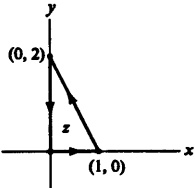
\includegraphics[width=0.20\textwidth]{figures/ch4_img_in_image_box_404_245_599_433.jpg}
\end{center}

\item Let  $ \alpha = (2x + y \cos xy)dx + (x \cos xy)dy $ on  $ \mathbb{R}^2 $. Show that  $ \alpha $ is closed. Show that  $ \alpha $ is exact by finding a function  $ f $:  $ \mathbb{R}^2 \to \mathbb{R} $ with  $ \alpha = df $. What would the integral of  $ \alpha $ over the cycle of Exercise 13 be?

\item Let

\[
\alpha=\frac{1}{2\pi}\frac{x\,dy-y\,dx}{x^{2}+y^{2}}.
\]

Prove that $\alpha$ is a closed 1-form on $\mathbb{R}^2 - \{0\}$. Compute the integral of $\alpha$ over the unit circle $S^1$. How does this result show that $\alpha$ is not exact? How does this show that $\delta i(\alpha)$ is not exact, where $i: S^1 \to \mathbb{R}^2$ is the canonical imbedding?

\item (a) Prove that every closed 1-form on  $ S^{2} $ is exact.

(b) Let

\[
\sigma=\frac{r_{1}\,d r_{2}\wedge d r_{3}-r_{2}\,d r_{1}\wedge d r_{3}+r_{3}\,d r_{1}\wedge d r_{2}}{(r_{1}^{2}+r_{2}^{2}+r_{3}^{2})^{3/2}}
\]

in  $ \mathbb{R}^{3} - \{0\} $. Prove that  $ \sigma $ is closed.

(c) Evaluate  $ \int_{S^{2}}\sigma $. How does this show that  $ \sigma $ is not exact?

(d) Let

\[
\alpha=\frac{r_{1}d r_{1}+r_{2}d r_{2}+\cdots+r_{n}d r_{n}}{(r_{1}^{2}+r_{2}^{2}+\cdots+r_{n}^{2})^{n/2}}
\]

in  $ \mathbb{R}^n - \{0\} $. Find  $ *\alpha $, and prove that  $ *\alpha $ is closed.

(e) Evaluate  $ \int_{S^{n-1}} \ast \alpha $. Is  $ \ast \alpha $ exact?

\item Using de Rham cohomology, prove that the torus $T^{2}$ is not diffeomorphic with the 2-sphere $S^{2}$.

\item (a) Prove that every closed 1-form in the open shell

\[
1<\left(\sum_{i=1}^{3}r_{i}^{2}\right)^{1/2}<2
\]

in $\mathbb{R}^{3}$ is exact.

(b) Find a 2-form in the above shell that is closed but not exact.

(c) Prove that the above shell is not diffeomorphic with the open unit ball in  $ \mathbb{R}^{3} $.

\item Let $f$ and $g$ be $C^\infty$ maps of $M$ into $N$ which are $C^\infty$ homotopic; that is, there exists a $C^\infty$ map $F$ of $M \times(-\varepsilon,1+\varepsilon)$ into $N$, for some $\varepsilon>0$, such that $F(m,0)=f(m)$ and $F(m,1)=g(m)$ for every $m\in M$. Prove that the induced homomorphisms $f^*$ and $g^*$ of $H_{\mathrm{de\,R}}^{p}(N)$ into $H_{\mathrm{de\,R}}^{p}(M)$ are equal for each integer $p$. (Hint: You will need to prove that the two injections $i_{0}(m)=(m,0)$ and $i_{1}(m)=(m,1)$ of $M$ into $M\times(-\varepsilon,1+\varepsilon)$ induce the same homomorphisms on de Rham cohomology. To prove this, find suitable homotopy operators. The outline of the proof of the Poincaré \hyperref[thm:4.18]{lemma 4.18} should be helpful.)

\item (a) Let $f: M^n \to \mathbb{R}^{n+1}$ be an immersion, and let $M^n$ be given the induced Riemannian structure; that is, for $m \in M$ and $u, v \in M_m$,

\[
\langle u,v\rangle_{m}=\langle d f(u),d f(v)\rangle_{f(m)}.
\]

Suppose that $M$ is oriented, and that $\vec{n}$ is the oriented unit normal field along $f(M^n)$. (This means that $\vec{n}, df(v_1), \ldots, df(v_n)$ is to be an oriented orthonormal basis of the tangent space to Euclidean space at $f(m)$ whenever $v_1, \ldots, v_n$ is an oriented orthonormal basis of $M_m$.) Show that the volume form on $M$ is given by

\[
\omega=\delta f\big(i(\vec{n})(dr_{1}\wedge\cdots\wedge dr_{n+1})\big).
\]

(b) Let $D$ be an open set in the xy plane, and let $\varphi: D \to \mathbb{R}^3$ be a smooth map of the form

\[
\varphi(x,y)=\bigl(x,y,f(x,y)\bigr).
\]

Thus $\varphi$ determines an imbedded surface in $\mathbb{R}^{3}$. Give $D$ and $\mathbb{R}^{3}$ the standard orientations. Use part (a) to prove that the induced volume form on $D$ is given by

\[
\omega=\left(\sqrt{\left(\frac{\partial f}{\partial x}\right)^{2}+\left(\frac{\partial f}{\partial y}\right)^{2}+1}\right)\,dx\wedge dy.
\]

\end{problemset}
